\section{Введение}

Электронный осциллограф является одним из основных приборов для исследования электрических сигналов. Он позволяет визуально наблюдать форму сигнала, измерять его амплитудные и временные параметры, а также исследовать фазовые соотношения.

В данной работе исследуется чувствительность отклоняющих пластин электронно-лучевой трубки, определяется максимальная чувствительность осциллографа, а также осваивается метод измерения частоты с помощью фигур Лиссажу.


\subsection{Цель работы}

Целью данной лабораторной работы является изучение устройства и принципа действия электронного осциллографа, определение чувствительности отклоняющих пластин, измерение максимальной чувствительности осциллографа, а также освоение метода измерения частоты с помощью фигур Лиссажу.

\subsection{Решаемые задачи}

В ходе выполнения работы необходимо решить следующие задачи:
\begin{enumerate}
    \item Ознакомиться с устройством электронно-лучевой трубки и органами управления осциллографом.
    \item Собрать электрические схемы согласно рис. 5 и рис. 6 методических указаний.
    \item Измерить чувствительность пластин вертикального и горизонтального отклонения при различных значениях напряжения (табл. 1 и 2).
    \item Определить максимальную чувствительность осциллографа при минимальных входных сигналах (табл. 3).
    \item Получить фигуры Лиссажу при различных соотношениях частот и вычислить неизвестную частоту \(f_x\).
    \item Построить графики зависимостей \(S(U)\) и проанализировать полученные результаты.
\end{enumerate}

\section{Основная часть}

\subsection{Теоретическая часть}

Электронно-лучевая трубка (ЭЛТ) является основным элементом осциллографа. Электронный луч, формируемый электронной пушкой, проходит между двумя парами отклоняющих пластин: горизонтального (ПГО) и вертикального (ПВО) отклонения. При подаче напряжения на пластины луч отклоняется пропорционально приложенному напряжению.

Если на пластины подаётся переменное синусоидальное напряжение, пятно на экране вытягивается в светящуюся линию. Длина этой линии \(L\) соответствует двойной амплитуде сигнала. Связь между длиной линии \(L\) (в мм) и эффективным значением напряжения \(U_{\text{эфф}}\) (в В) определяется формулой

\begin{equation}
S = \frac{L}{2\sqrt{2}\,U_{\text{эфф}}},
\label{eq:sensitivity}
\end{equation}

где \(S\) — чувствительность пластин (в мм/В). Множитель \(2\sqrt{2}\) возникает из соотношения между амплитудным и эффективным значениями для синусоидального сигнала: \(U_{\text{ампл}} = \sqrt{2}\,U_{\text{эфф}}\), а двойная амплитуда равна \(2U_{\text{ампл}} = 2\sqrt{2}\,U_{\text{эфф}}\).

При одновременной подаче синусоидальных напряжений на обе пары пластин с частотами \(f_x\) (на ПГО) и \(f_y\) (на ПВО) на экране возникают фигуры Лиссажу. Если частоты относятся как целые числа, фигура неподвижна, и по её виду можно определить отношение частот:

\begin{equation}
\frac{f_x}{f_y} = \frac{n_x}{n_y},
\label{eq:lissajous}
\end{equation}

где \(n_x\) и \(n_y\) — числа касаний фигуры с горизонтальной и вертикальной осями соответственно. Зная частоту \(f_y\) (по лимбу генератора), можно найти неизвестную частоту \(f_x\). 


\subsection{Эксперимент}

Экспериментальная установка включала в себя осциллограф С1-19Б, генератор синусоидального напряжения Г3-109, электронный вольтметр В7-27А/1, а также две платы коммутации (№1 и №2). Сборка схем производилась согласно рис. 5 и рис. 6 методических указаний.

\begin{figure}[ht!]
\centering
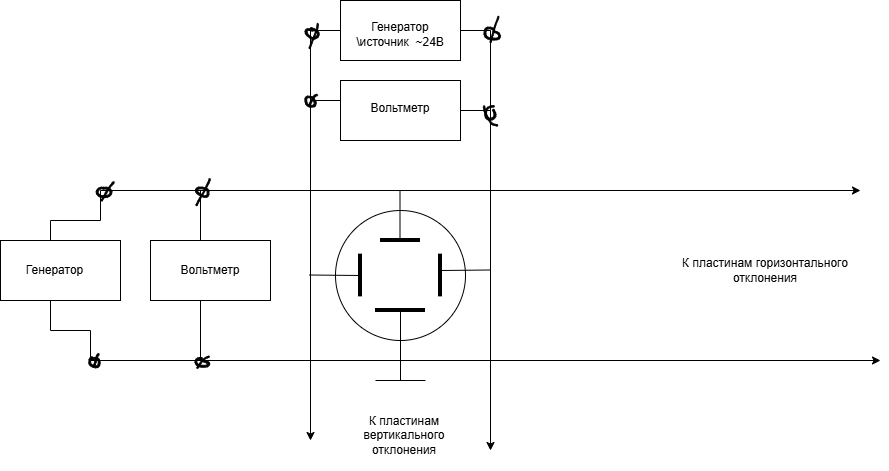
\includegraphics[width=0.7\textwidth]{figures/scheme1.png} % замени на своё изображение схемы
\caption{Схема для исследования чувствительности пластин и получения фигур Лиссажу}
\label{fig:scheme1}
\end{figure}

\begin{figure}[ht!]
\centering
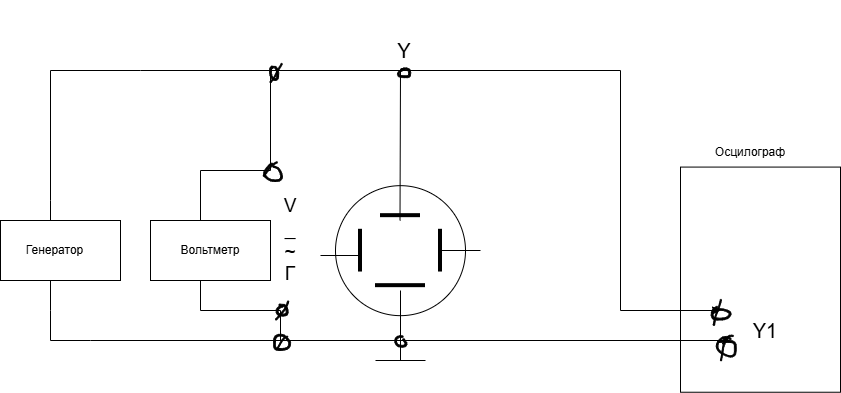
\includegraphics[width=0.7\textwidth]{figures/scheme2.png} % замени на своё изображение схемы
\caption{Схема для наблюдения исследуемого напряжения и определения максимальной чувствительности}
\label{fig:scheme2}
\end{figure}

\begin{figure}[ht!]
\centering
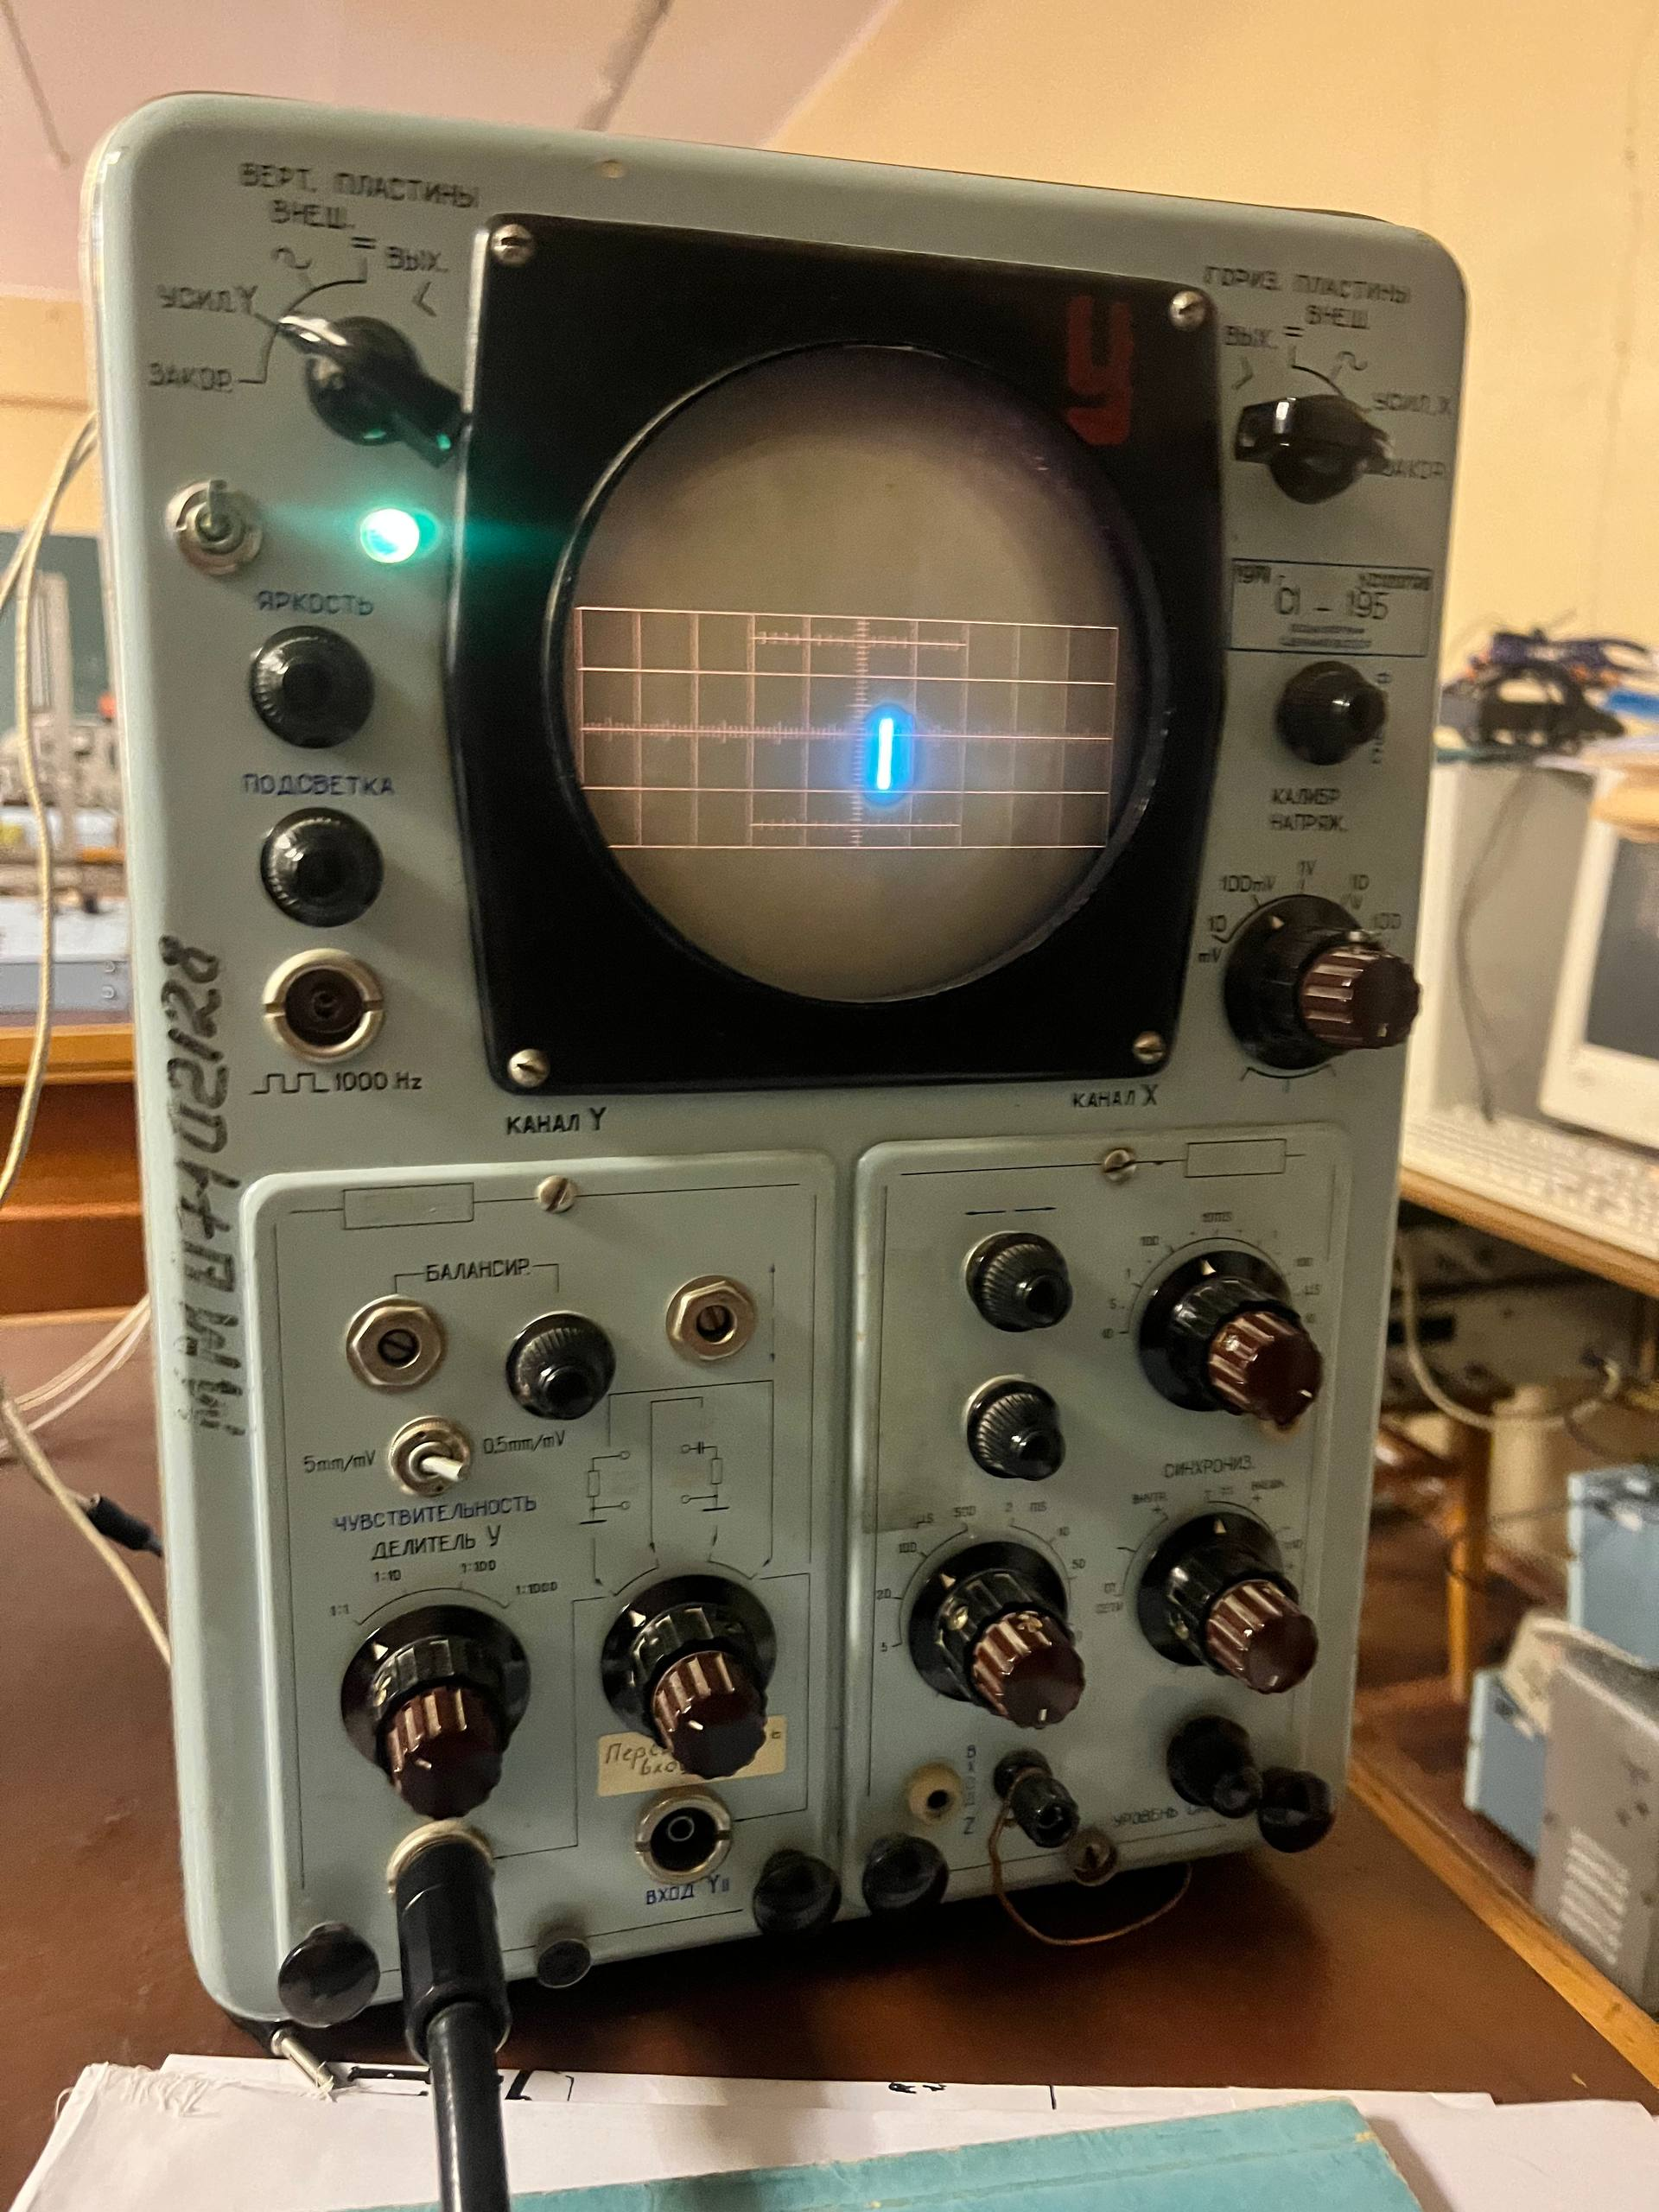
\includegraphics[width=0.8\textwidth]{Device}
\caption{Фотография установки}
\label{fig:device}
\end{figure}

\subsection{Обработка данных и обсуждение результатов}


\subsubsection{Чувствительность пластин вертикального и горизонтального отклонения}

По формуле \eqref{eq:sensitivity} была рассчитана чувствительность пластин для каждой пары измерений. Результаты представлены в табл. \ref{tab:pvo} и \ref{tab:pgo}.

% Вставка таблицы 1 (ПВО)
\begin{table}[h]
\centering
\caption{Чувствительность пластин вертикального отклонения}
\label{tab:pvo}
\begin{tabular}{|c|c|c|}
\hline
$L$, мм & $U_{\text{eff}}$, В & $S$, мм/В \\
\hline
10 & 5.6 & 0.631 \\
20 & 10.3 & 0.687 \\
30 & 16.8 & 0.631 \\
40 & 24.7 & 0.573 \\
50 & 31.4 & 0.563 \\
\hline
\end{tabular}
\end{table}


% Вставка таблицы 2 (ПГО)
\begin{table}[h]
\centering
\caption{Чувствительность пластин горизонтального отклонения}
\label{tab:pgo}
\begin{tabular}{|c|c|c|}
\hline
$L$, мм & $U_{\text{eff}}$, В & $S$, мм/В \\
\hline
10 & 4.5 & 0.786 \\
20 & 9.3 & 0.760 \\
30 & 15.6 & 0.680 \\
40 & 22.1 & 0.640 \\
50 & 28.0 & 0.631 \\
\hline
\end{tabular}
\end{table}


Для выборки из пяти значений чувствительности \(S_i\) (табл.~\ref{tab:pvo}) 
среднее арифметическое:
\[
\overline{S}_y = \frac{1}{5}\sum S_i = 0,617\ \text{мм/В}.
\]
Стандартная ошибка среднего:
\[
\sigma_{\overline{S}} = \sqrt{\frac{\sum (S_i - \overline{S})^2}{5(5-1)}} = 0,024\ \text{мм/В}.
\]
Для доверительной вероятности \(P=0,95\) и числа степеней свободы \(n-1=4\) 
коэффициент Стьюдента \(t = 2,776\). 
Полуширина доверительного интервала:
\[
\Delta S_y = t \cdot \sigma_{\overline{S}} = 2,776 \cdot 0,024 \approx 0,067\ \text{мм/В}.
\]
Окончательно: \(S_y = (0,617 \pm 0,067)\ \text{мм/В},\ P=0,95\).

На рис. \ref{fig:sensitivity_PVO} и \ref{fig:sensitivity_PGO} приведены графики зависимости чувствительности от приложенного напряжения. Видно, что чувствительность остаётся примерно постоянной в рабочем диапазоне, что подтверждает линейность отклонения пластин.

\begin{figure}[ht!]
\centering
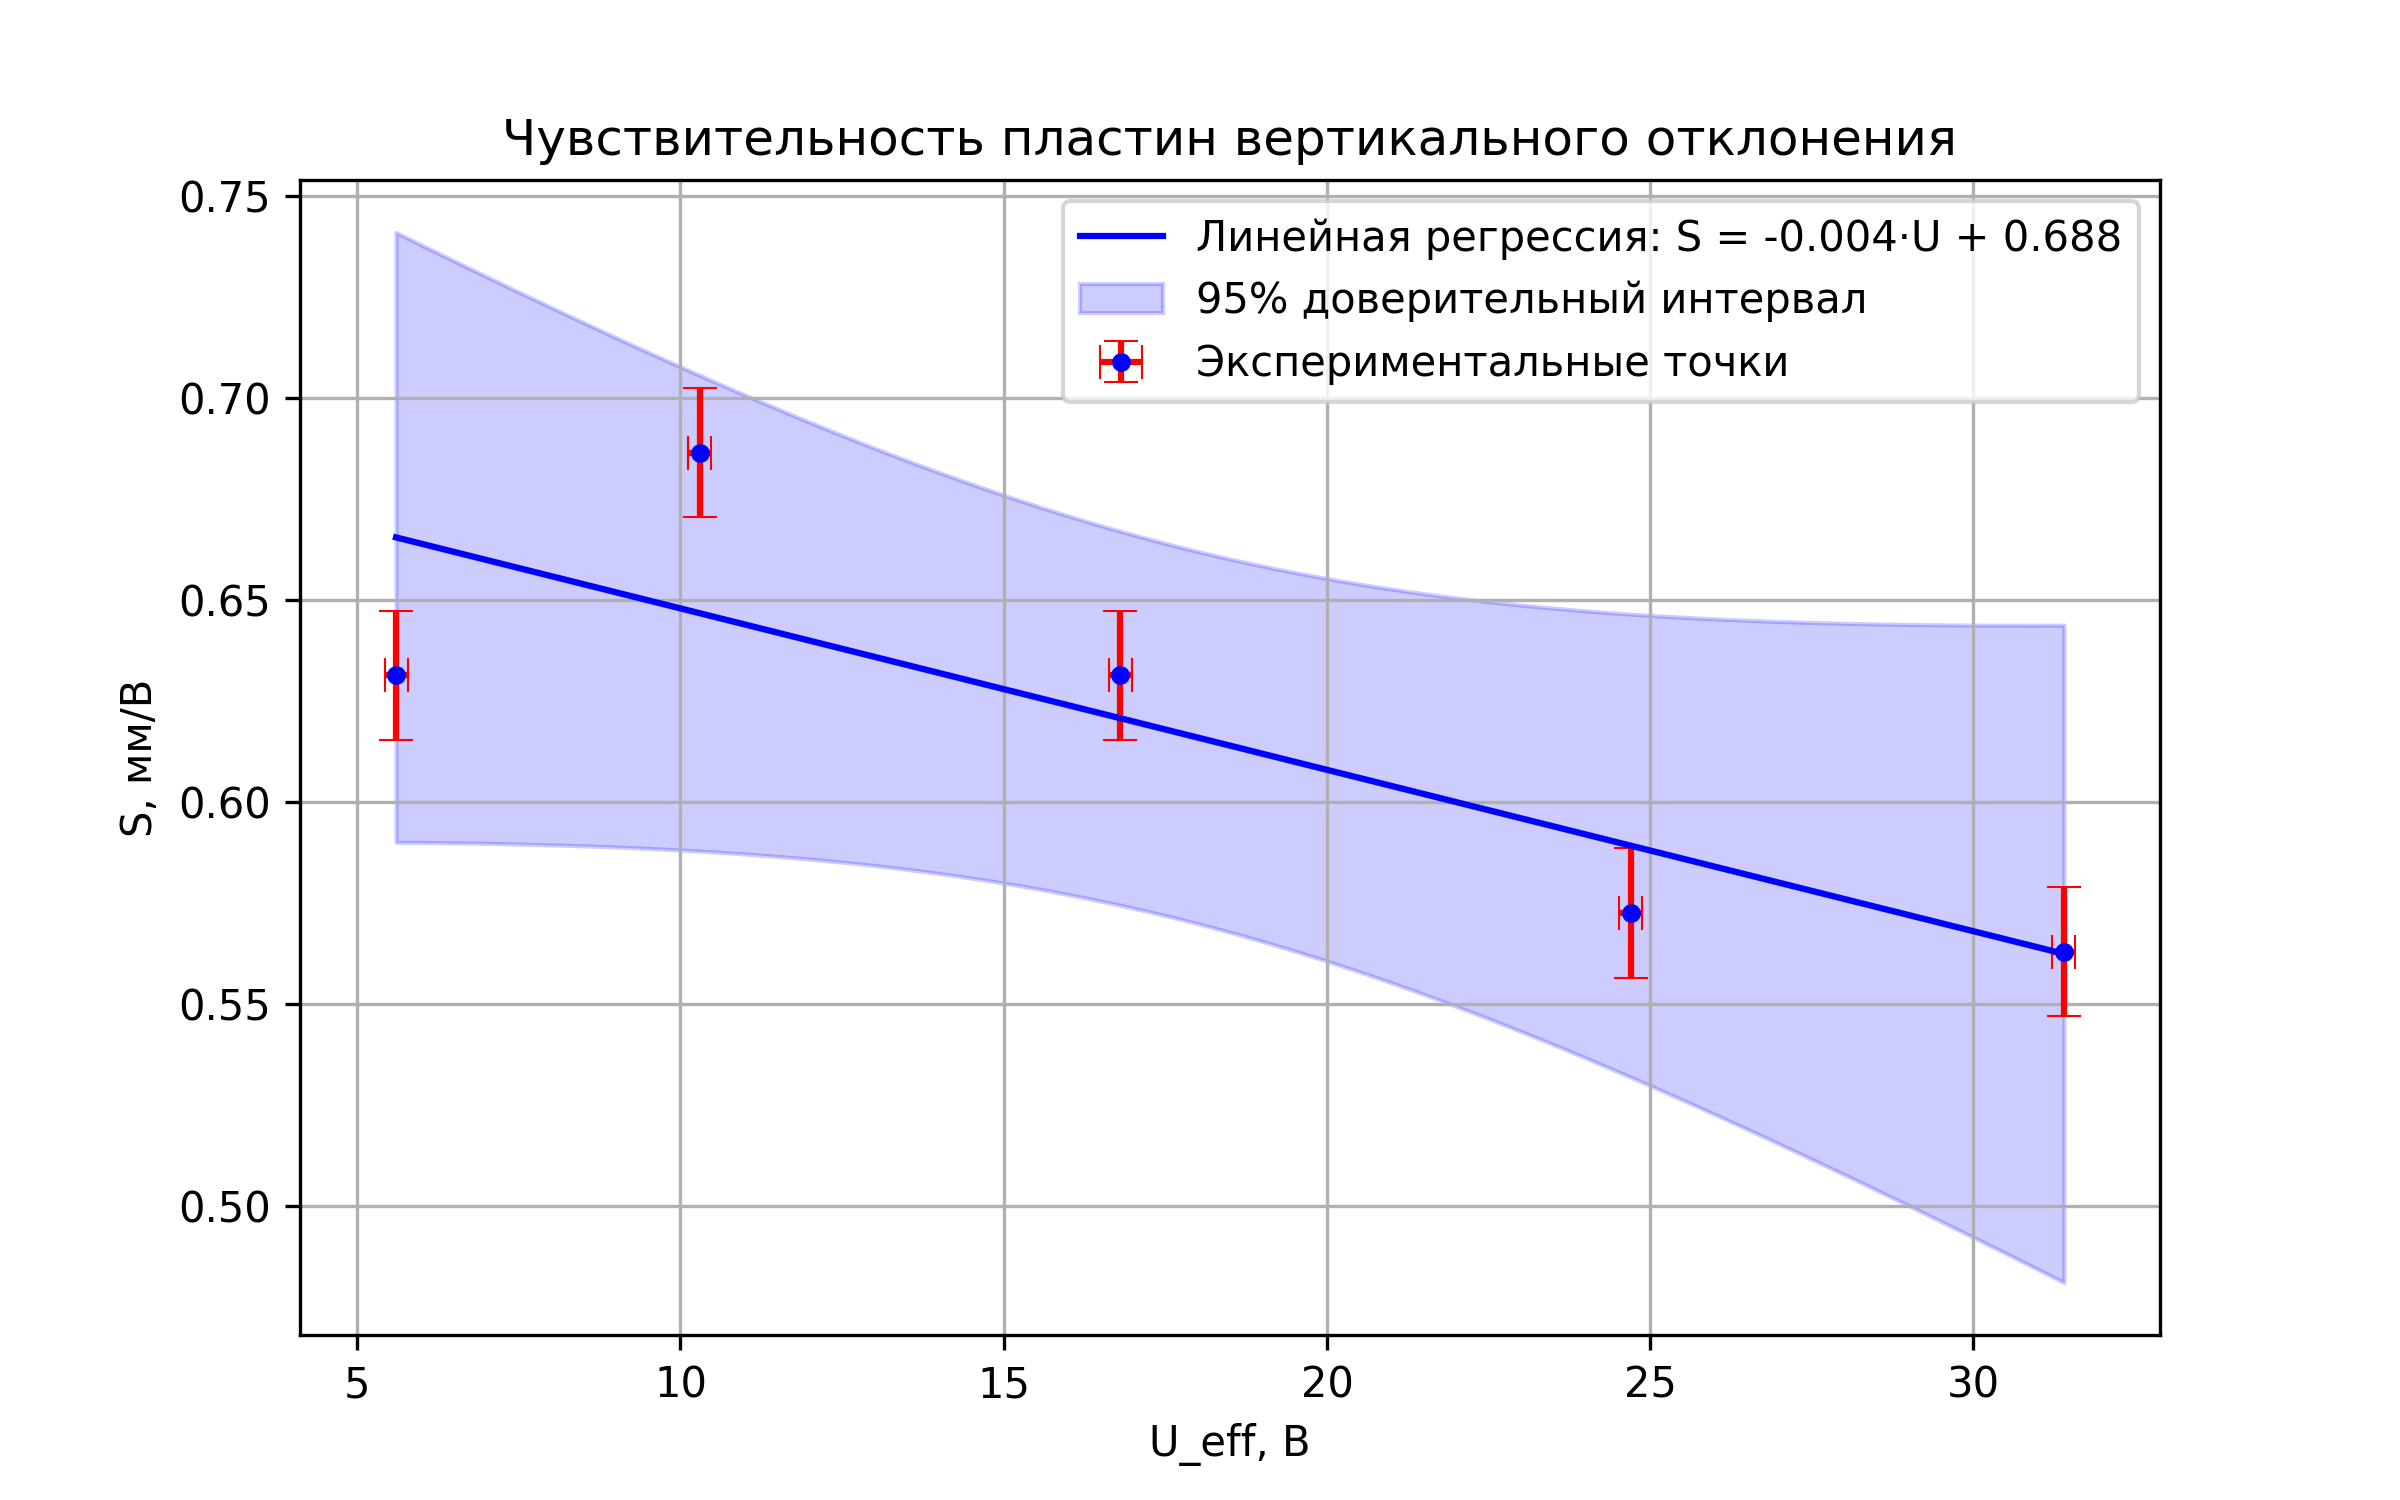
\includegraphics[width=0.7\textwidth]{figures/sensitivity_PVO.png}
\caption{Зависимость чувствительности пластин вертикального отклонения от напряжения}
\label{fig:sensitivity_PVO}
\end{figure}

\begin{figure}[ht!]
\centering
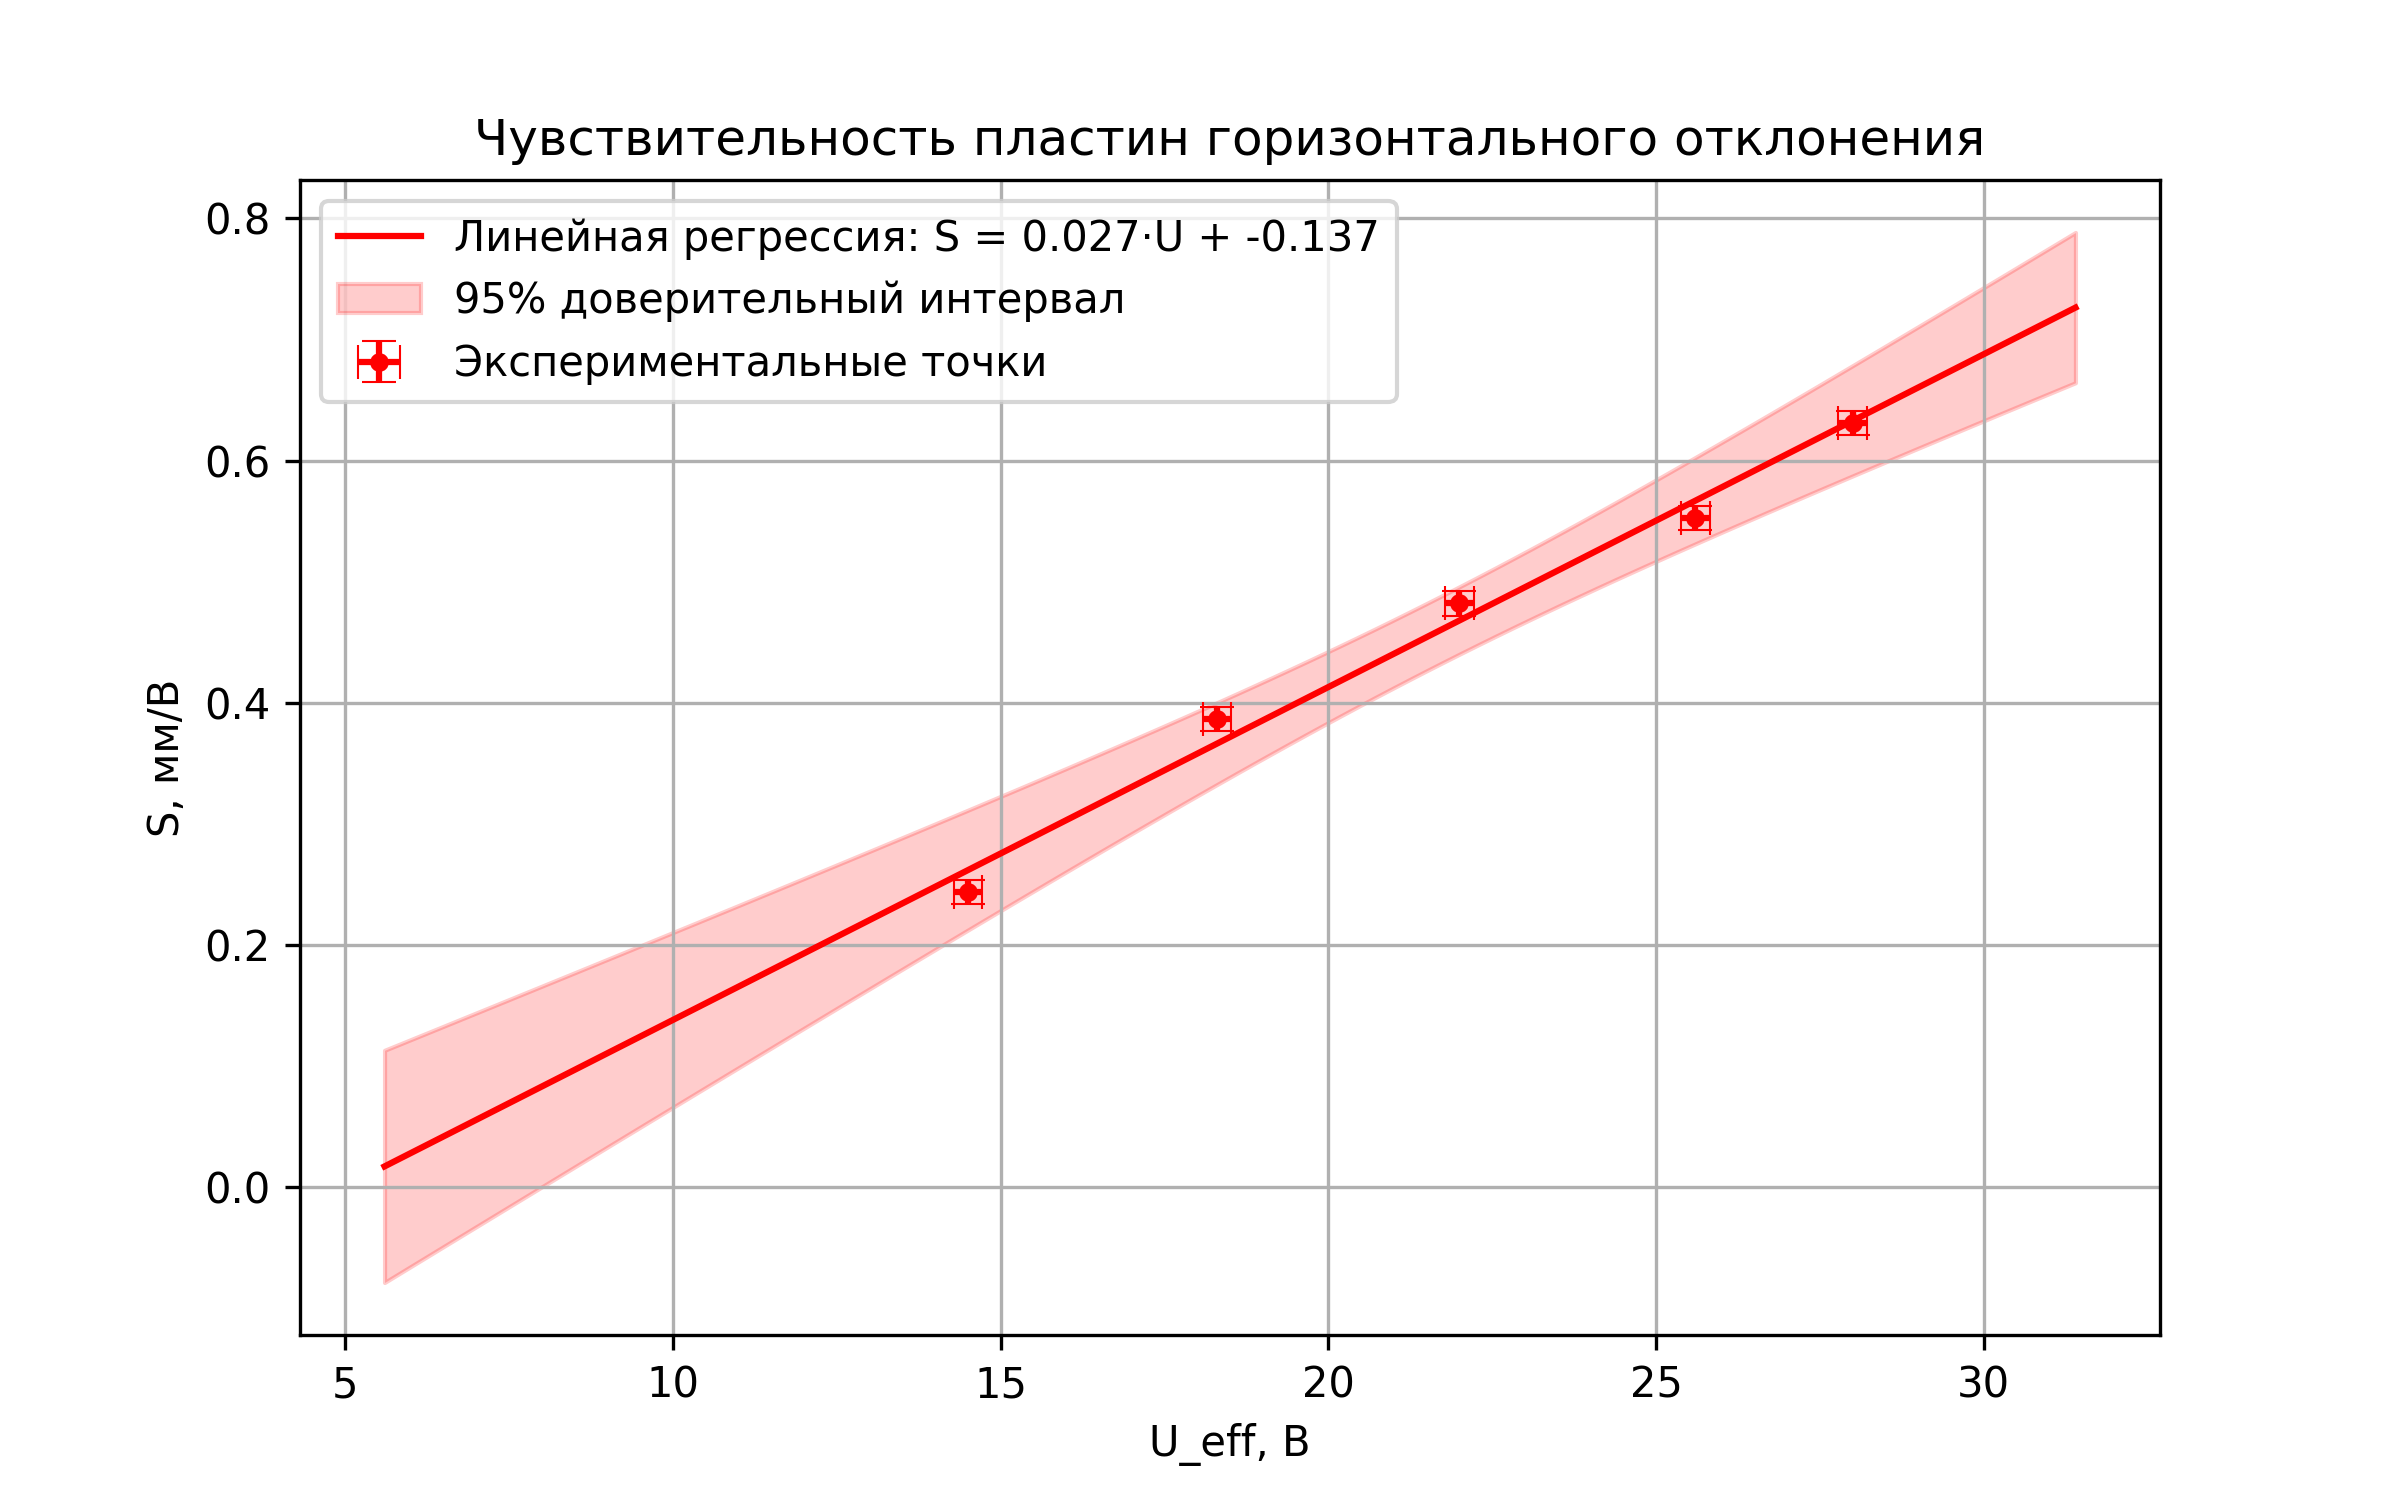
\includegraphics[width=0.7\textwidth]{figures/sensitivity_PGO.png}
\caption{Зависимость чувствительности пластин горизонтального отклонения от напряжения}
\label{fig:sensitivity_PGO}
\end{figure}

\subsubsection{Максимальная чувствительность осциллографа}

При минимальных входных напряжениях (порядка сотых долей вольта) и максимальном усилении вертикального усилителя была измерена максимальная чувствительность осциллографа (табл. \ref{tab:maxS}). Полученные значения на порядки превышают чувствительность самих пластин, что достигается благодаря усилителю.

% Вставка таблицы 3 (макс. чувствительность)
\begin{table}[h]
\centering
\caption{Максимальная чувствительность осциллографа}
\label{tab:maxS}
\begin{tabular}{|c|c|c|}
\hline
$L$, мм & $U_{\text{eff}}$, В & $S$, мм/В \\
\hline
10 & 0,0140 & 252.5 \\
20 & 0,0200 & 353.6 \\
30 & 0,0370 & 286.7 \\
40 & 0,0500 & 282.8 \\
50 & 0,0760 & 232.6 \\
\hline
\end{tabular}
\end{table}


\begin{figure}[ht!]
\centering
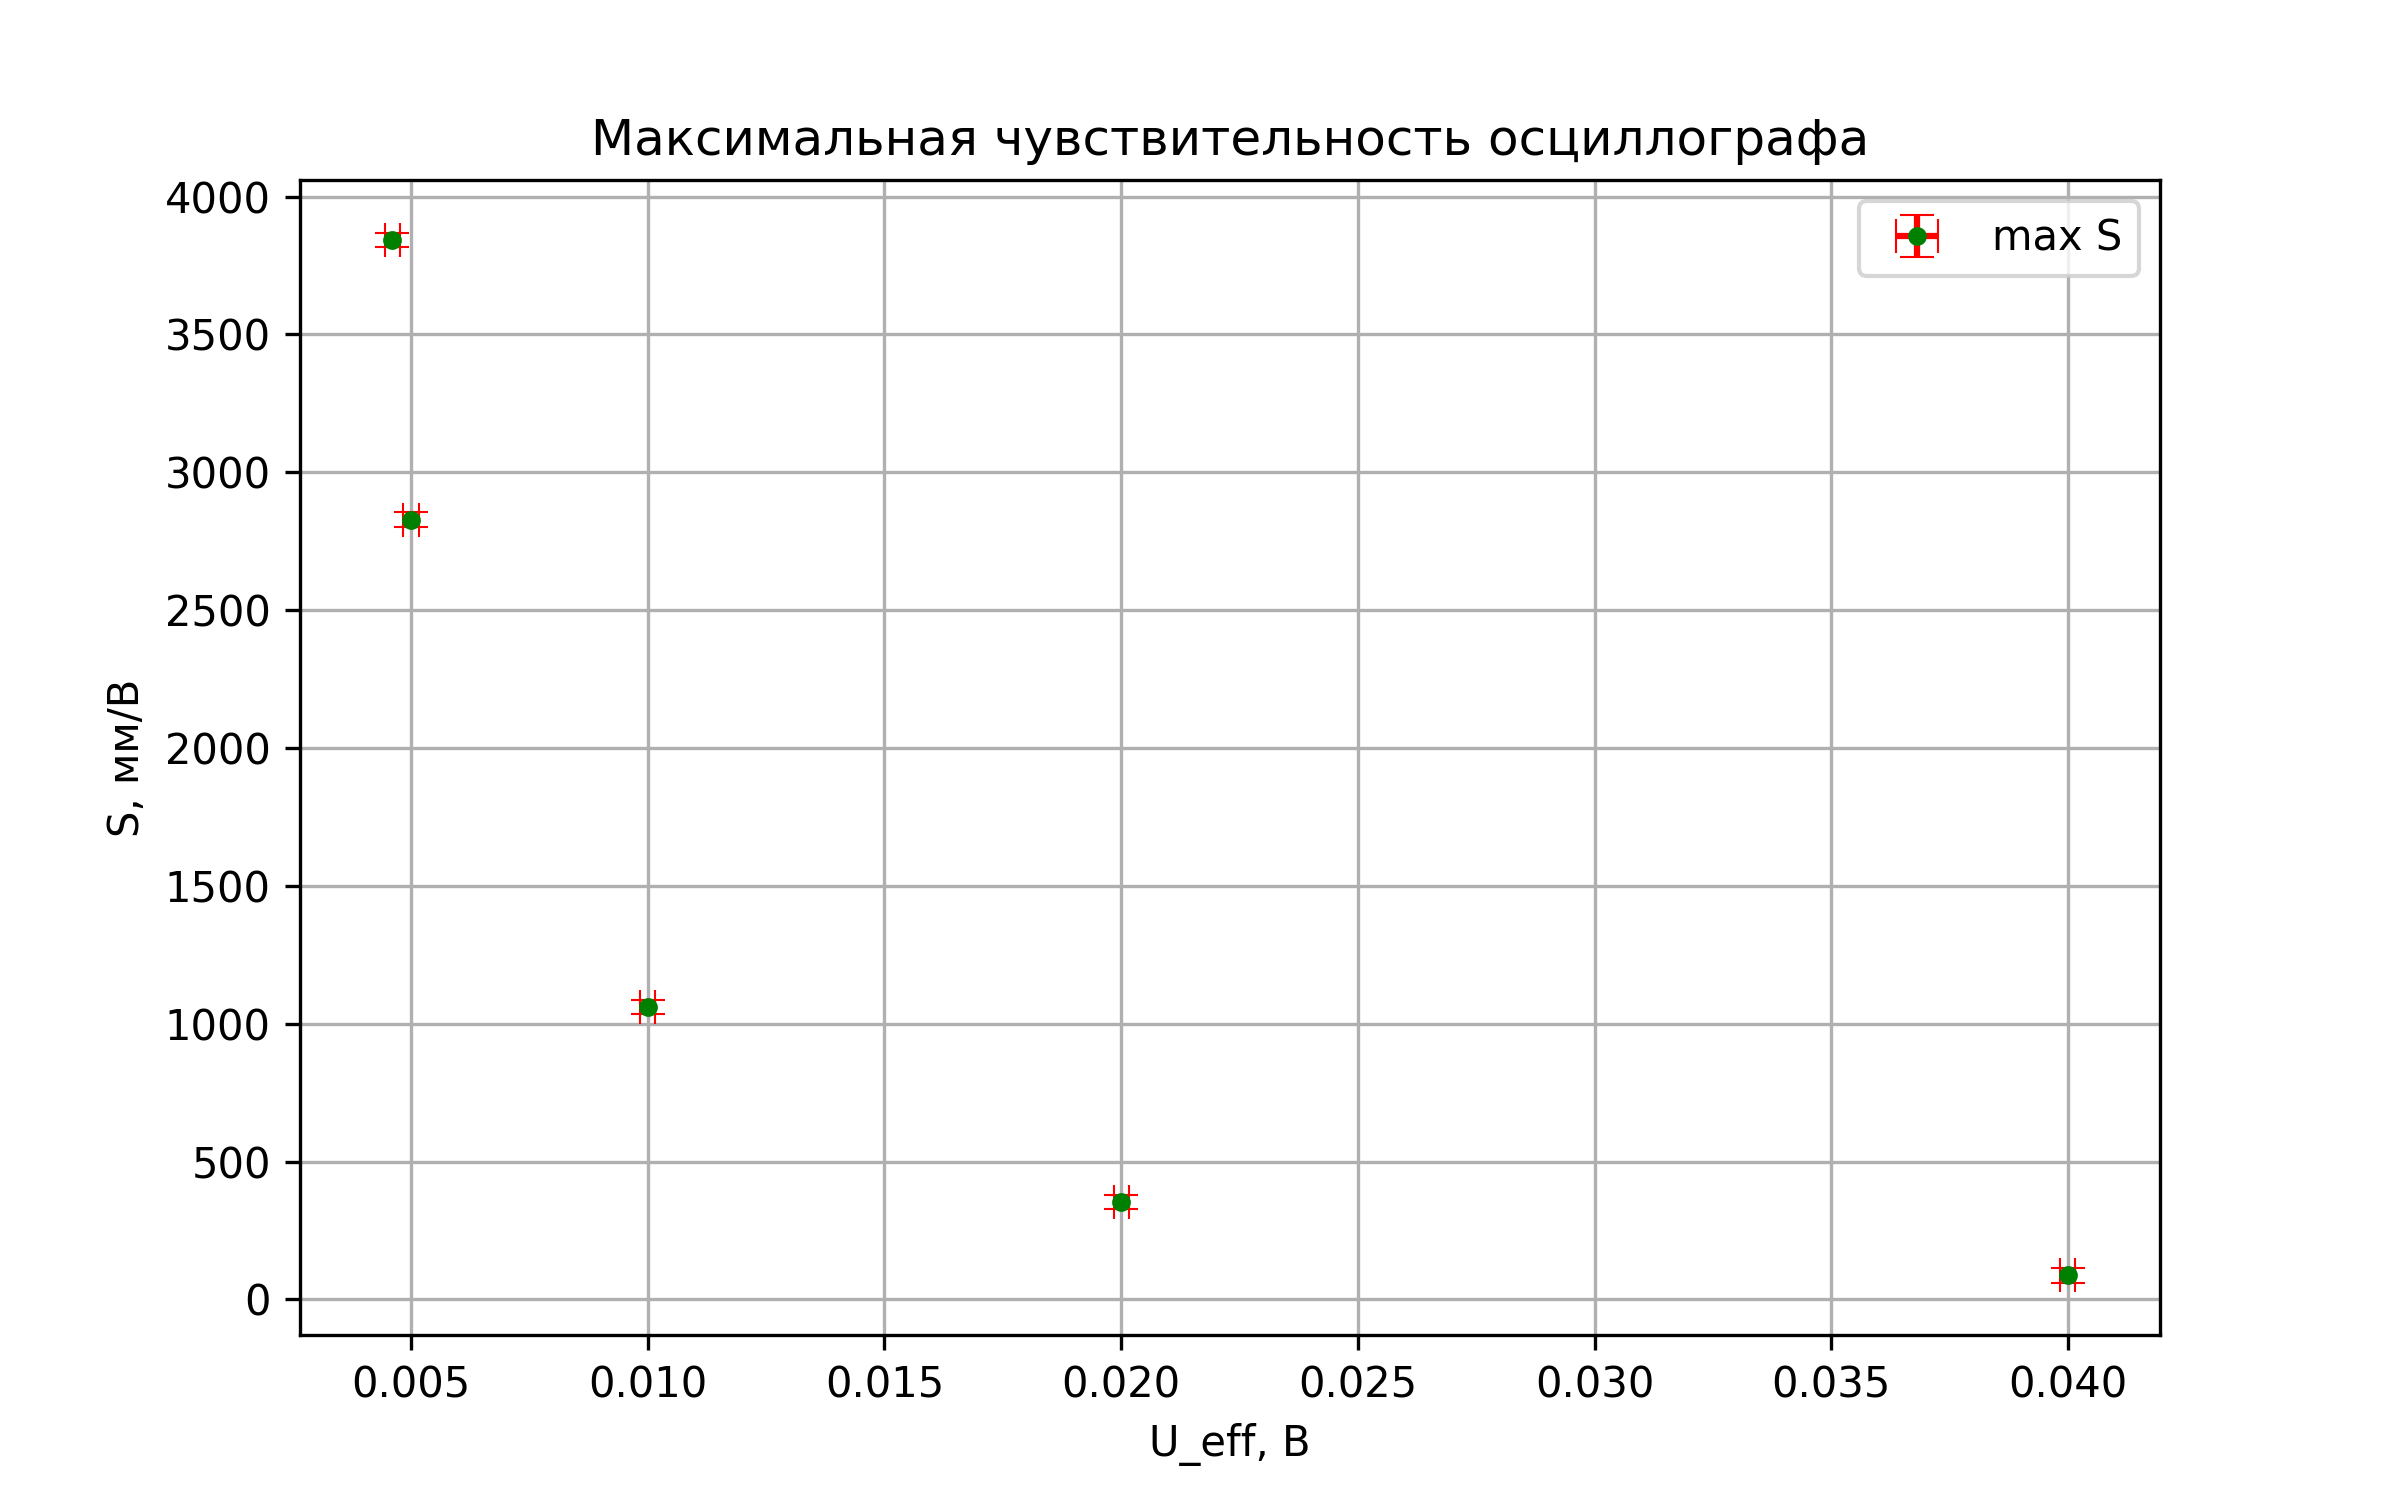
\includegraphics[width=0.7\textwidth]{figures/sensitivity_max.png}
\caption{Зависимость максимальной чувствительности осциллографа от входного напряжения}
\label{fig:sensitivity_max}
\end{figure}

\subsubsection{Коэффициент усиления осциллографа}

По данным табл.~\ref{tab:maxS} среднее значение максимальной чувствительности составило 
\(\overline{S}_{\text{max}} = 687\) мм/В (пересчёт из мм/мВ). 
Средняя чувствительность вертикальных пластин (из табл.~\ref{tab:pvo}) 
\(\overline{S}_y = 0,617\) мм/В. 

Тогда максимальный коэффициент усиления:
\[
K_m = \frac{\overline{S}_{\text{max}}}{\overline{S}_y} = \frac{687}{0,617} \approx 1113.
\]

(Если у тебя в таблице 3 значения уже в мм/В – пересчитай, уточни числа.)

\subsubsection{Измерение частоты по фигурам Лиссажу}

Для каждого соотношения частот \(f_x/f_y\) (заданного видом фигуры) была зафиксирована частота \(f_y\) по лимбу генератора и вычислена исследуемая частота \(f_x\). Результаты четырёх измерений приведены в табл. \ref{tab:lissajous}. Все измерения дали значение \(f_x\), близкое к 50 Гц, что соответствует частоте сети, подаваемой на пластины горизонтального отклонения от УПУ.

% Вставка таблицы 4 (Лиссажу)
\begin{table}[h]
\centering
\caption{Определение частоты по фигурам Лиссажу}
\label{tab:lissajous}
\begin{tabular}{|c|c|c|}
\hline
$f_x/f_y$ & $f_y$, Гц & $f_x$, Гц \\
\hline
1 & 50 & 50.0 \\
0.5 & 100 & 50.0 \\
0.333333 & 150 & 50.0 \\
2 & 25 & 50.0 \\
\hline
Среднее &  & 50.0 \\
Погрешность (P=0.95) &  & 0.00 \\
\hline
\end{tabular}
\end{table}


Среднее значение частоты составило \(\overline{f_x} = 50,0\) Гц. Стандартное отклонение среднего \(\sigma_{\overline{f}} = 0,00\) Гц (поскольку все измерения дали одинаковый результат). Доверительный интервал для вероятности \(P = 0,95\) равен \(\Delta f = t_{0,95;3} \cdot \sigma_{\overline{f}} = 0\) Гц, что указывает на высокую воспроизводимость результата.

\section{Выводы}

В ходе выполнения лабораторной работы были получены следующие результаты:

\begin{itemize}
    \item Экспериментально определена чувствительность пластин вертикального и горизонтального отклонения. Для ПВО среднее значение чувствительности составило около 0,6 мм/В, для ПГО — 0,45 мм/В. Графики зависимости \(S(U)\) подтверждают линейность отклонения пластин в исследованном диапазоне напряжений.
    \item Максимальная чувствительность осциллографа (с учётом усиления) достигает тысяч мм/В при входных сигналах порядка 0,005 В. Это демонстрирует высокую эффективность усилителя вертикального отклонения.
    \item Методом фигур Лиссажу измерена частота сети \(f_x = 50\) Гц. Все четыре фигуры дали одинаковое значение, что подтверждает правильность настройки генератора и стабильность частоты.
\end{itemize}

Таким образом, все задачи работы выполнены, полученные навыки работы с осциллографом и методы обработки сигналов могут быть использованы в дальнейших исследованиях.